\documentclass[sigconf]{acmart}

\usepackage{booktabs}
\usepackage{multirow}
\usepackage{amsmath}
\usepackage{graphicx}

\setcopyright{none}
\settopmatter{printacmref=false}
\renewcommand\footnotetextcopyrightpermission[1]{}
\pagestyle{plain}

\begin{document}

\title{Query-Sample Sensitivity and Cross-Lingual Rank Transfer for Pairwise LLM-as-a-Judge Evaluation in Multilingual RAG}

\author{Devarasetty Seetesh}
\affiliation{%
  \institution{IT Department, Indian Institute of Information Technology-Allahabad}
  \city{Prayagraj}
  \country{India}
}
\email{MRA2026015@iiita.ac.in}

\begin{abstract}
Automated pairwise evaluation using Large Language Models (LLMs) as judges can introduce reliability issues when static leaderboards are constructed from limited query budgets or single-language benchmarks. Variations in evaluation sample size and target language can alter the relative ordering of candidate Retrieval-Augmented Generation (RAG) systems.

Three evaluation methodologies were tested to examine how pairwise model rankings behave under controlled query subsampling and cross-lingual transfer: (M1) full-sample pairwise win-rate aggregation, (M2) query-grouped bootstrap and repeated subsampling across $25\%$, $50\%$, $75\%$, and $100\%$ query budgets, and (M3) cross-lingual pairwise rank correlation across 18 languages. The MIRAGE-Bench pairwise judgment benchmark (\texttt{nthakur/mirage-bench-pairwise-judgments}) was used, containing $299{,}119$ validated pairwise verdicts across 19 models and 18 languages.

A query-grouped protocol was enforced with fixed random seeds (\texttt{42} and \texttt{123}), ensuring all $\binom{19}{2} = 171$ model comparisons per query remained intact without partial-query leakage. Win rates, ordinal ranks, rank standard deviations, empirical $95\%$ confidence intervals, Kendall's $\tau_b$, and Spearman's $\rho$ were calculated.

On the English development set (100 queries; $17{,}097$ judgments), proprietary frontier models achieved the highest win rates (\texttt{gpt-4o-azure}: $0.8533$; \texttt{gpt-4-azure}: $0.8419$), followed by \texttt{Meta-Llama-3-70B-Instruct} ($0.7017$). Under repeated subsampling ($R=100$), mean Kendall's $\tau_b$ increased from $0.8552 \pm 0.0492$ at $25\%$ queries to $0.9174 \pm 0.0315$ at $50\%$ and $0.9516 \pm 0.0210$ at $75\%$. However, while top- and bottom-tier models stabilized completely ($\text{SD} = 0.000$ at $75\%$ queries), mid-tier open-weight models exhibited substantial rank churn ($\text{SD} = 1.453$ for \texttt{Mistral-7B-Instruct-v0.2}). Across all 153 language pairs, cross-lingual correlation averaged $\tau_b = 0.6921 \pm 0.1121$ ($\rho = 0.8366 \pm 0.0947$), dropping sharply between English and lower-resource languages such as Telugu (\texttt{en}--\texttt{te}: $\tau_b = 0.3801$) and Swahili (\texttt{en}--\texttt{sw}: $\tau_b = 0.4386$).
\end{abstract}

\keywords{Retrieval-Augmented Generation, LLM-as-a-Judge, Pairwise Evaluation, Ranking Stability, Multilingual NLP, MIRAGE-Bench}

\maketitle

\section{Introduction}
Reliable evaluation is essential in Retrieval-Augmented Generation (RAG) research, enabling practitioners to compare candidate language models on faithfulness and answer quality~\cite{lewis2020rag,gao2023rag}. Automated pairwise evaluation---termed \textit{LLM-as-a-judge}---presents two candidate responses to an automated judge and aggregates categorical verdicts (\texttt{A}, \texttt{B}, or \texttt{Tie}) into scalar leaderboards~\cite{zheng2023judging,chiang2024chatbot}.

This workflow relies on two critical assumptions: (1) compact query subsets preserve true model orderings despite $\binom{M}{2}$ pairwise matchups per query, and (2) rankings derived on English benchmarks transfer reliably to typologically diverse and lower-resource languages~\cite{thakur2024mirage}. This study investigates both assumptions across 19 models and 18 languages.

\subsection{Objectives}
\begin{itemize}
    \item Establish a verified baseline win-rate ranking of 19 LLMs on the English MIRAGE-Bench development partition.
    \item Quantify how query-budget reduction ($25\%, 50\%, 75\%$) affects leaderboard stability and empirical confidence intervals.
    \item Identify which model capability tiers experience the highest rank volatility under small query budgets.
    \item Measure cross-lingual rank transfer across 18 languages to expose divergences between high- and low-resource evaluation settings.
\end{itemize}

\subsection{Research Questions}
\begin{itemize}
    \item \textbf{RQ1:} What is the baseline win-rate hierarchy of the 19 evaluated LLMs on the English MIRAGE-Bench development partition?
    \item \textbf{RQ2:} How does reducing the evaluation query budget ($25\%, 50\%, 75\%$) affect overall ranking correlation (Kendall's $\tau_b$) and per-model rank stability?
    \item \textbf{RQ3:} Do pairwise model rankings derived on English transfer consistently across all 18 languages in MIRAGE-Bench?
\end{itemize}

\section{Related Work}
Prior surveys categorize hallucination mechanisms in generative language models~\cite{ji2023survey,huang2025survey}, while benchmarks such as RAGTruth~\cite{niu2024ragtruth}, HaluEval~\cite{li2023halueval}, FActScore~\cite{min2023factscore}, and RAGAS~\cite{es2024ragas} evaluate factual grounding. Pairwise LLM-as-a-judge frameworks~\cite{zheng2023judging,chiang2024chatbot} improve agreement over pointwise scoring, though Wang et al.~\cite{wang2024large} document systematic judge biases and Voorhees~\cite{voorhees2002trec} highlights sample-size sensitivity in retrieval rankings. Thakur et al.~\cite{thakur2024mirage} introduced MIRAGE-Bench across 18 languages; we extend this evidence base with controlled query-subsampling stability and exhaustive cross-lingual rank correlation analysis.

\section{Dataset and Experimental Setup}
We use the MIRAGE-Bench pairwise judgments dataset (\texttt{nthakur/mirage-bench-pairwise-judgments})~\cite{thakur2024mirage}, comprising $299{,}119$ validated pairwise comparisons across 18 languages and 19 candidate models (Table~\ref{tab:lang_summary}). All records were validated by dropping null fields in \texttt{query\_id}, \texttt{model\_A}, \texttt{model\_B}, and \texttt{verdict}, trimming whitespace, and restricting labels strictly to $\{\texttt{A}, \texttt{B}, \texttt{Tie}\}$. Subsampling partitions were constructed strictly at the \texttt{query\_id} level with fixed seeds (\texttt{42} and \texttt{123}) so all $\binom{19}{2} = 171$ comparisons per query stayed intact.

\begin{table}[t]
\centering
\caption{Validated Dataset Statistics and Top Model Across 18 Languages}
\label{tab:lang_summary}
\scriptsize
\begin{tabular}{lcccc}
\toprule
\textbf{Lang.} & \textbf{Records} & \textbf{Queries} & \textbf{Top-1 Model} & \textbf{Win Rate} \\
\midrule
\texttt{ar} & 17,099 & 100 & \texttt{gpt-4-azure} & 0.8900 \\
\texttt{bn} & 17,099 & 100 & \texttt{gpt-4o-azure} & 0.9156 \\
\texttt{de} & 17,099 & 100 & \texttt{gpt-4o-azure} & 0.8997 \\
\texttt{en} & 17,097 & 100 & \texttt{gpt-4o-azure} & 0.8533 \\
\texttt{es} & 17,086 & 100 & \texttt{gpt-4o-azure} & 0.8750 \\
\texttt{fa} & 8,717  & 51  & \texttt{gpt-4o-azure} & 0.9106 \\
\texttt{fi} & 17,084 & 100 & \texttt{gpt-4o-azure} & 0.8774 \\
\texttt{fr} & 17,098 & 100 & \texttt{gpt-4-azure} & 0.9105 \\
\texttt{hi} & 17,057 & 100 & \texttt{gpt-4-azure} & 0.9121 \\
\texttt{id} & 17,095 & 100 & \texttt{gpt-4-azure} & 0.8544 \\
\texttt{ja} & 17,096 & 100 & \texttt{gpt-4o-azure} & 0.8519 \\
\texttt{ko} & 17,096 & 100 & \texttt{gpt-4o-azure} & 0.8519 \\
\texttt{ru} & 17,050 & 100 & \texttt{gpt-4-azure} & 0.8556 \\
\texttt{sw} & 16,992 & 100 & \texttt{gpt-4o-azure} & 0.9040 \\
\texttt{te} & 17,099 & 100 & \texttt{gpt-4o-azure} & 0.8992 \\
\texttt{th} & 17,097 & 100 & \texttt{gpt-4o-azure} & 0.8767 \\
\texttt{yo} & 17,100 & 100 & \texttt{gpt-4-azure} & 0.8775 \\
\texttt{zh} & 17,096 & 100 & \texttt{gpt-4o-azure} & 0.8747 \\
\bottomrule
\end{tabular}
\end{table}

\section{Methodology}
Figure~\ref{fig:workflow} summarizes the end-to-end experimental workflow.

\begin{figure*}[t]
\centering
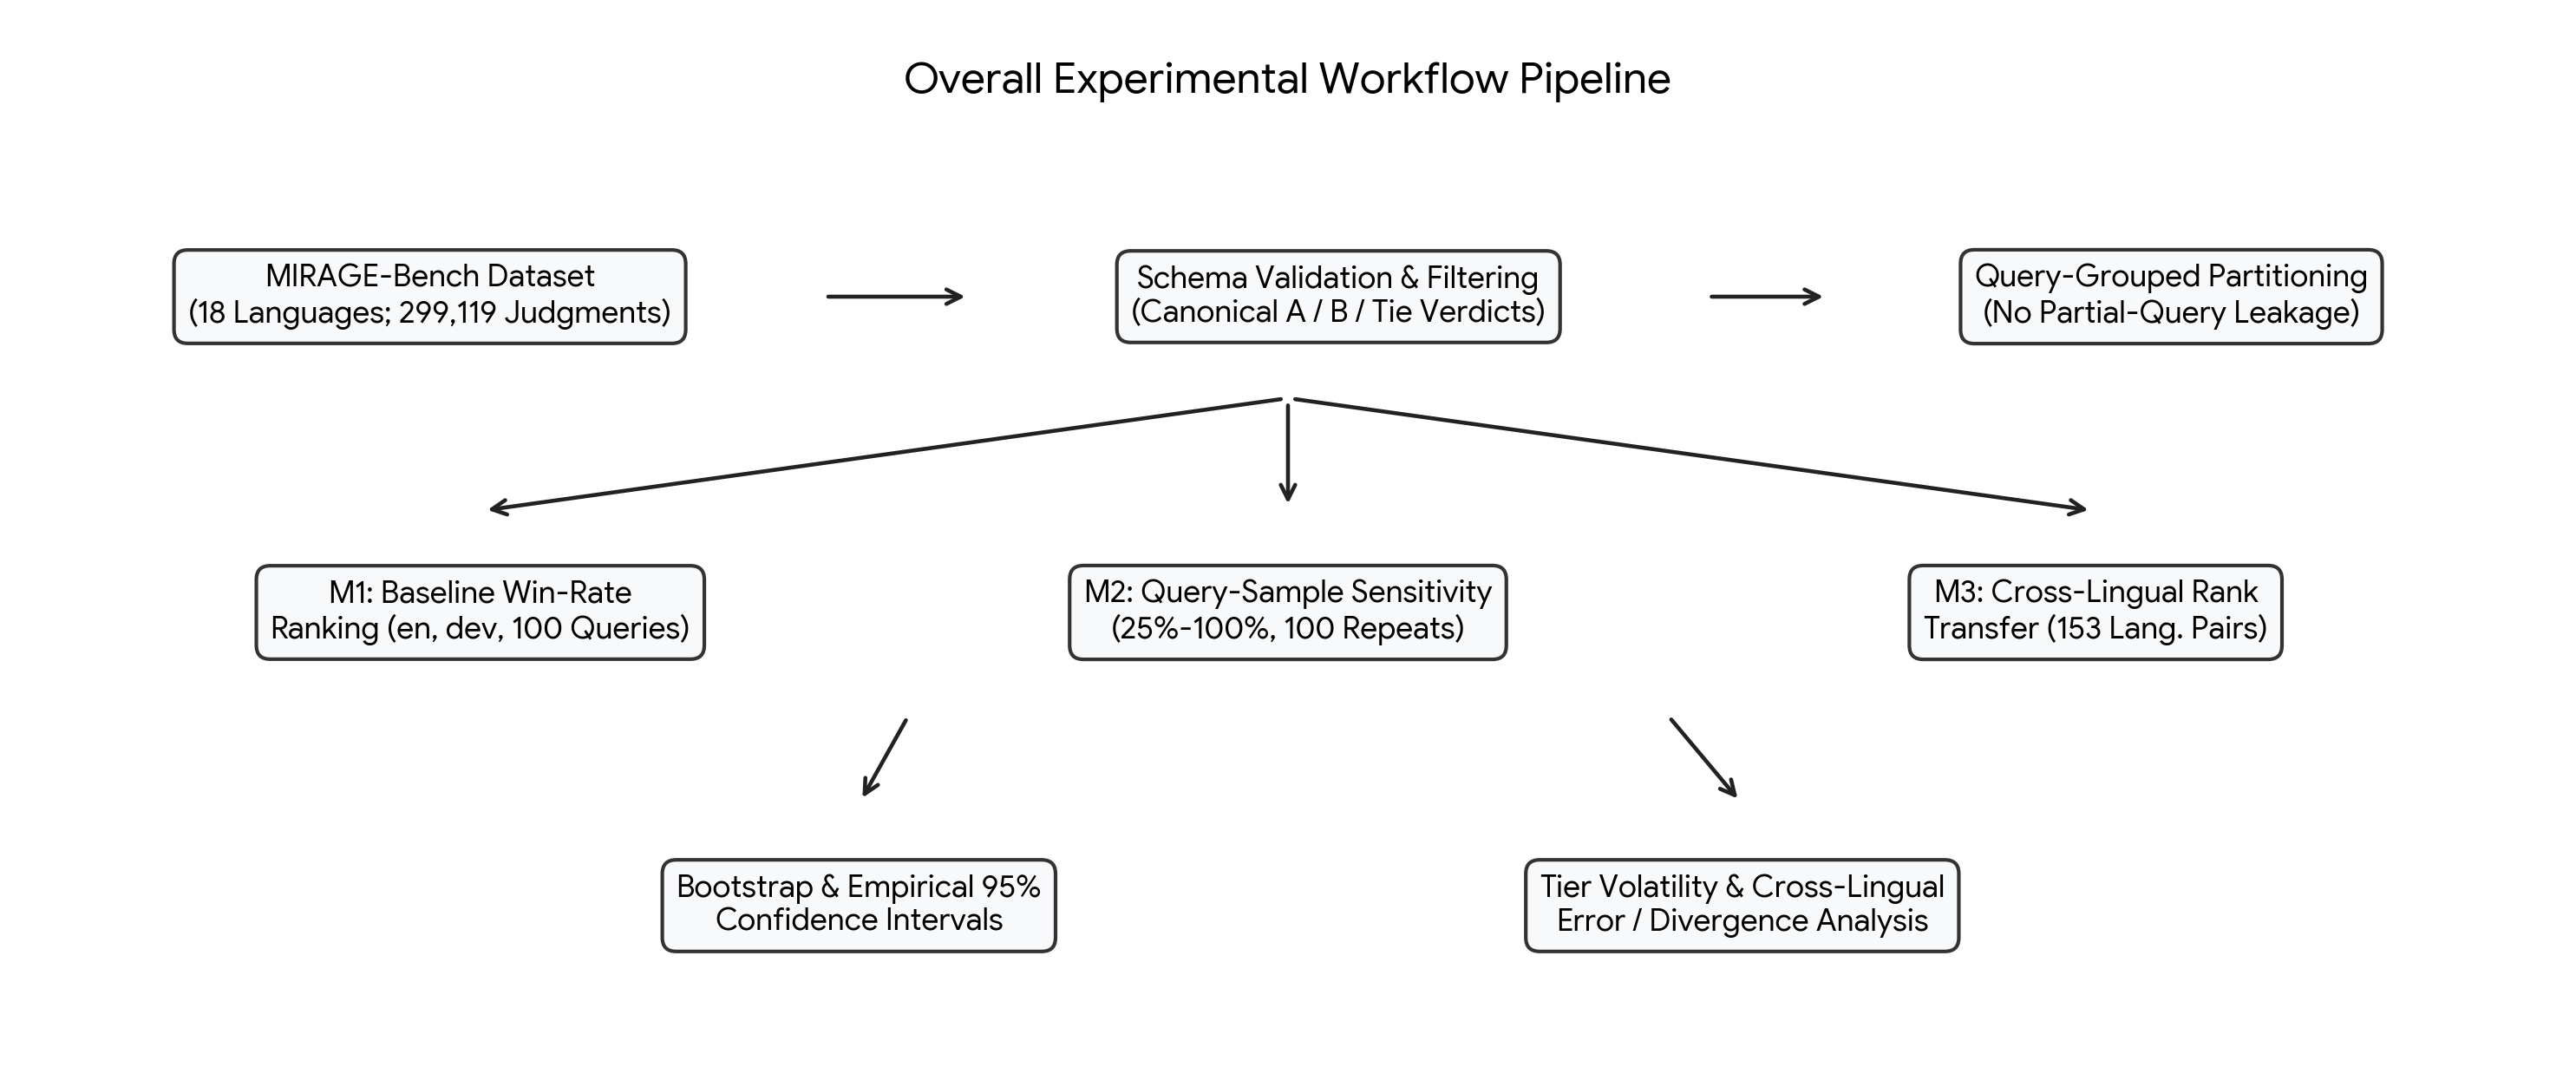
\includegraphics[width=0.90\textwidth]{fig1_workflow_pipeline.png}
\caption{Overall experimental workflow pipeline for pairwise LLM-as-a-judge ranking stability and cross-lingual transfer.}
\label{fig:workflow}
\end{figure*}

\subsection{Method 1 (M1): Pairwise Win-Rate Aggregation}
For each model $m \in \mathcal{M}$ ($M = 19$), wins $W_m$, losses $L_m$, ties $T_m$, and total comparisons $N_m = W_m + L_m + T_m$ are accumulated across all head-to-head judgments. With tie weight $w_{\text{tie}} = 0.5$:
\begin{equation}
\text{WinRate}(m) = \frac{W_m + 0.5 \, T_m}{N_m}
\label{eq:winrate}
\end{equation}

\subsection{Method 2 (M2): Query-Sample Sensitivity and Bootstrap Protocol}
On English ($|\mathcal{Q}| = 100$), we perform: (1) $B = 100$ bootstrap resamples with replacement (\texttt{seed=42}), and (2) $R = 100$ repeated subsamples without replacement (\texttt{seed=42}) at query fractions $f \in \{0.25, 0.50, 0.75, 1.00\}$, plus per-model rank tracking (\texttt{seed=123}) across $R = 100$ repeats.

\subsection{Method 3 (M3): Cross-Lingual Rank Transfer}
Independent win-rate vectors $\mathbf{w}^{(\ell)}$ are computed for all 18 languages, and rank correlations are evaluated across all $\binom{18}{2} = 153$ unordered language pairs.

\section{Evaluation Metrics}
We evaluate rankings using Kendall's $\tau_b$ (tie-adjusted ordinal concordance), Spearman's $\rho$ (monotonic rank correlation), per-model rank standard deviation $\text{SD}_m$, and empirical $95\%$ percentile intervals $[q_{0.025}, q_{0.975}]$:
\begin{equation}
\tau_b = \frac{P - Q}{\sqrt{(P + Q + T_x)(P + Q + T_y)}}, \qquad \rho = 1 - \frac{6 \sum_{i=1}^{M} (r_{x,i} - r_{y,i})^2}{M(M^2 - 1)}
\label{eq:corr}
\end{equation}

\section{Experimental Results}
Tables~\ref{tab:en_ranking}--\ref{tab:lang_corr} and Figure~\ref{fig:ranking_stability} present the experimental results across RQ1, RQ2, and RQ3.

\begin{table}[t]
\centering
\caption{Baseline Pairwise Model Ranking on English (\texttt{en}, \texttt{dev} Split)}
\label{tab:en_ranking}
\scriptsize
\begin{tabular}{clcccc}
\toprule
\textbf{Rank} & \textbf{Model} & \textbf{Wins} & \textbf{Losses} & \textbf{Ties} & \textbf{Win Rate} \\
\midrule
1  & \texttt{gpt-4o-azure} & 1,423 & 151 & 226 & 0.8533 \\
2  & \texttt{gpt-4-azure} & 1,392 & 161 & 247 & 0.8419 \\
3  & \texttt{Meta-Llama-3-70B-Instruct} & 1,124 & 398 & 278 & 0.7017 \\
4  & \texttt{Mixtral-8x22B-Instruct-v0.1} & 996 & 505 & 299 & 0.6364 \\
5  & \texttt{Qwen2-7B-Instruct} & 871 & 645 & 283 & 0.5628 \\
6  & \texttt{Phi-3-small-8k-instruct} & 843 & 657 & 300 & 0.5517 \\
7  & \texttt{Mixtral-8x7B-Instruct-v0.1} & 862 & 729 & 209 & 0.5369 \\
8  & \texttt{cohereforai-c4ai-command-r} & 844 & 793 & 162 & 0.5142 \\
9  & \texttt{cohereforai-c4ai-aya-23} & 765 & 779 & 256 & 0.4961 \\
10 & \texttt{cohereforai-c4ai-command-r-plus} & 718 & 820 & 262 & 0.4717 \\
11 & \texttt{Mistral-7B-Instruct-v0.3} & 692 & 829 & 279 & 0.4619 \\
12 & \texttt{Mistral-7B-Instruct-v0.2} & 711 & 870 & 217 & 0.4558 \\
13 & \texttt{Phi-3-medium-128k-instruct} & 630 & 826 & 344 & 0.4456 \\
14 & \texttt{gpt-3.5-turbo-azure} & 676 & 873 & 250 & 0.4452 \\
15 & \texttt{Meta-Llama-3-8B-Instruct} & 655 & 926 & 218 & 0.4247 \\
16 & \texttt{gemma-1.1-7b-it} & 518 & 1,004 & 278 & 0.3650 \\
17 & \texttt{Phi-3-mini-128k-instruct} & 421 & 1,154 & 225 & 0.2964 \\
18 & \texttt{gemma-1.1-2b-it} & 394 & 1,299 & 107 & 0.2486 \\
19 & \texttt{Qwen2-1.5B-Instruct} & 248 & 1,364 & 188 & 0.1900 \\
\bottomrule
\end{tabular}
\end{table}

\begin{table}[t]
\centering
\caption{Ranking Stability (Kendall's $\tau_b$) Across Query Sample Fractions ($R = 100$ Repeats)}
\label{tab:stability_summary}
\scriptsize
\begin{tabular}{cccccc}
\toprule
\textbf{Frac.} & \textbf{Queries} & \textbf{Mean $\tau_b$} & \textbf{SD} & \textbf{Min--Max} & \textbf{95\% Interval} \\
\midrule
0.25 & 25  & 0.8552 & 0.0492 & 0.7193--0.9649 & [0.7465, 0.9415] \\
0.50 & 50  & 0.9174 & 0.0315 & 0.8363--0.9766 & [0.8480, 0.9766] \\
0.75 & 75  & 0.9516 & 0.0210 & 0.8947--0.9883 & [0.9064, 0.9883] \\
1.00 & 100 & 1.0000 & 0.0000 & 1.0000--1.0000 & --- \\
\bottomrule
\end{tabular}
\end{table}

\begin{figure}[t]
\centering
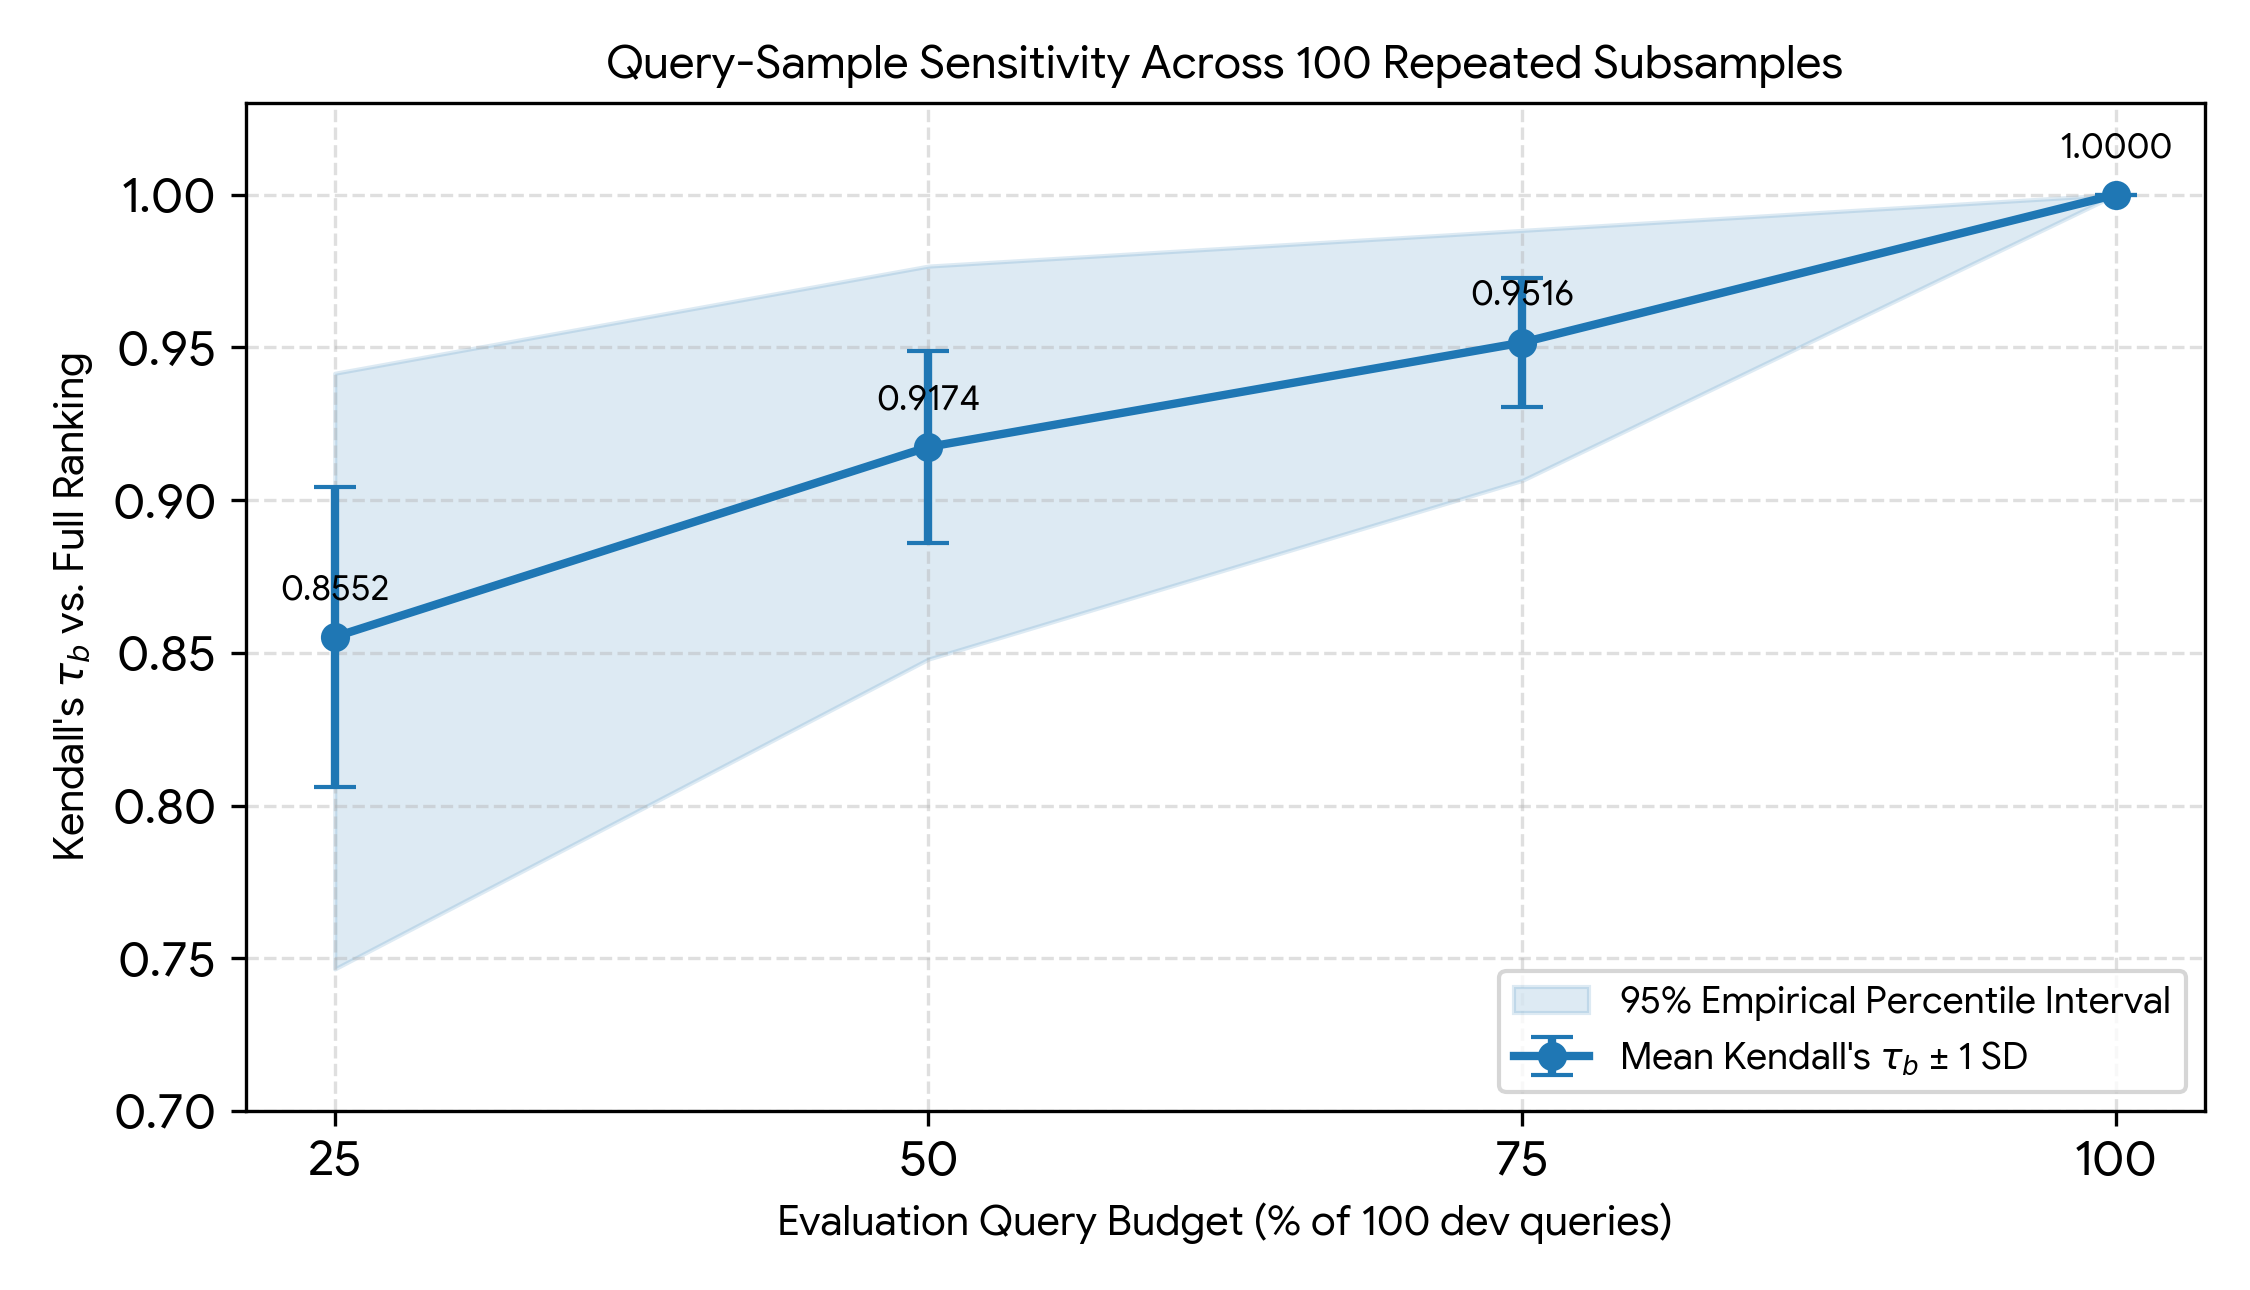
\includegraphics[width=\columnwidth]{fig2_ranking_stability.png}
\caption{Mean Kendall's $\tau_b$ with $\pm 1\text{ SD}$ error bars and $95\%$ empirical intervals across query budgets.}
\label{fig:ranking_stability}
\end{figure}

\begin{table}[t]
\centering
\caption{Highest and Lowest Cross-Lingual Ranking Correlations (19 Common Models)}
\label{tab:lang_corr}
\scriptsize
\begin{tabular}{llcc}
\toprule
\textbf{Category} & \textbf{Language Pair} & \textbf{Kendall's $\tau_b$} & \textbf{Spearman's $\rho$} \\
\midrule
\multirow{5}{*}{\textbf{Top-5 Pairs}}
 & \texttt{ja} -- \texttt{ko} & 1.0000 & 1.0000 \\
 & \texttt{ar} -- \texttt{id} & 0.9298 & 0.9860 \\
 & \texttt{es} -- \texttt{fr} & 0.9267 & 0.9873 \\
 & \texttt{fa} -- \texttt{hi} & 0.8830 & 0.9684 \\
 & \texttt{ar} -- \texttt{fa} & 0.8713 & 0.9649 \\
\midrule
\multirow{5}{*}{\textbf{Bottom-5 Pairs}}
 & \texttt{de} -- \texttt{te} & 0.3450 & 0.5088 \\
 & \texttt{en} -- \texttt{te} & 0.3801 & 0.5246 \\
 & \texttt{de} -- \texttt{th} & 0.4152 & 0.5807 \\
 & \texttt{bn} -- \texttt{de} & 0.4386 & 0.5842 \\
 & \texttt{en} -- \texttt{sw} & 0.4386 & 0.6000 \\
\bottomrule
\end{tabular}
\end{table}

\section{Discussion, Limitations, and Conclusion}
Our results demonstrate that while \texttt{gpt-4o-azure} and \texttt{gpt-4-azure} lead every language split, mid-tier open-weight models cluster within a compressed $0.1381$ win-rate band and suffer substantial rank churn at small query budgets ($\text{SD} = 2.69$ at $25\%$ queries for \texttt{Mistral-7B-Instruct-v0.2}). Across 153 language pairs, rank correlation averages $\tau_b = 0.6921 \pm 0.1121$ and drops sharply between English and lower-resource languages (\texttt{en}--\texttt{te}: $\tau_b = 0.3801$; \texttt{en}--\texttt{sw}: $\tau_b = 0.4386$). Limitations include reliance on a single automated judge, evaluation on 100-query development partitions, and equal tie weighting ($0.5$). Future work will incorporate parametric Bradley--Terry uncertainty intervals and multi-judge calibration.

\bibliographystyle{ACM-Reference-Format}
\bibliography{references}

\end{document}
